% TODO: give examples of theorem, lemmas, and proofs!
\documentclass[a4paper,twoside,11pt,hidelinks]{article}
\usepackage{a4wide,graphicx,fancyhdr,amsmath,amssymb,amsthm,ifthen,path}
\usepackage[ruled, noline, algo2e, noend]{algorithm2e}
\usepackage[hidelinks]{hyperref}
\usepackage{url}
\usepackage{color}
\usepackage{float}
\usepackage[section]{placeins}
\urlstyle{rm}

%----------------------- Macros and Definitions --------------------------

\setlength\headheight{20pt}
\addtolength\topmargin{-10pt}
\addtolength\footskip{20pt}

\newcommand{\N}{\ensuremath{\mathbb{N}}}
\newcommand{\R}{\ensuremath{\mathbb{R}}}
\newcommand{\Z}{\ensuremath{\mathbb{Z}}}
\newcommand{\ch}{\ensuremath{\mathcal{CH}}}

\fancypagestyle{plain}{%
\fancyhf{}
\fancyfoot[LO,RE]{\sffamily\bfseries 2IL55~--~Geometric Algorithms}
\fancyfoot[RO,LE]{\sffamily\bfseries\thepage}
\renewcommand{\headrulewidth}{0pt}
\renewcommand{\footrulewidth}{0pt}
}

\pagestyle{fancy}
\fancyhf{}
% ----------------------------------------------------------------------------
% Insert your names here:
% ----------------------------------------------------------------------------
\fancyhead[LE]{\sffamily\bfseries Daan Creemers, Pieter-Paul Kramer and Qi Xiao}
% ----------------------------------------------------------------------------
% Insert the title of your report here:
% ----------------------------------------------------------------------------
\fancyhead[RO]{\sffamily\bfseries Experimentation Project on Geometric t-Spanners}
%
\fancyfoot[LO,RE]{\sffamily\bfseries 2IL55~--~Geometric Algorithms}
\fancyfoot[RO,LE]{\sffamily\bfseries\thepage}
\renewcommand{\headrulewidth}{1pt}
\renewcommand{\footrulewidth}{0pt}

\theoremstyle{plain}
\newtheorem{definition}{Definition}
\newtheorem{theorem}{Theorem}
\newtheorem{lemma}{Lemma}
\newtheorem{proposition}{Proposition}
\newtheorem{corollary}{Corollary}
\newtheorem{fact}{Fact}
\theoremstyle{definition}  % switches off use of italics in following env's
\newtheorem{remark}{Remark}
\newtheorem{example}{Example}
% use \begin{proof}...\end{proof} for proofs (def'd in amsthm)

% set-up for algorithm2e
\SetArgSty{}
\setlength{\algomargin}{4ex}
\SetKw{KwOr}{or}
\SetKw{KwAnd}{and}
\SetKw{KwReturn}{return}
\SetKw{KwRequire}{Require:}
\SetKw{KwInvariant}{Invariant:}
\SetKwRepeat{KwRepeat}{repeat}{until}
%\dontprintsemicolon
% \linesnumbered

% Command 2: text to indent
\newcommand{\indented}[2] {
\begingroup
\leftskip#1
\rightskip\leftskip
#2
\par
\endgroup
}

%-------------------------------- Title ----------------------------------

\title{\sffamily\bfseries
% ----------------------------------------------------------------------------
% Insert the title of your report here:
% ----------------------------------------------------------------------------
Experimentation Project on Geometric t-Spanners \\[1ex]
%
\large Research report for Geometric Algorithms (2IL55) -- Autumn
semester 2014}

% ----------------------------------------------------------------------------
% Insert your names, student numbers, and email addresses here:
% ----------------------------------------------------------------------------
\author{
  \begin{minipage}[t]{.5\linewidth}
    \centering
    Daan Creemers \\
    Student number: 0748693 \\
    \texttt{d.j.a.creemers@student.tue.nl}
  \end{minipage}
  \begin{minipage}[t]{.5\linewidth}
    \centering
    Pieter-Paul Kramer \\
    Student number: 0675271 \\
    \texttt{p.kramer@student.tue.nl}
  \end{minipage}
  \\
  \begin{minipage}[t]{.5\linewidth}
    \centering
    \vspace{1em}
    Qi Xiao \\
    Student number: 0925490 \\
    \texttt{xiaqqaix@gmail.com}
  \end{minipage}
}

\hypersetup{%
  pdftitle={Experimentation Project on Geometric t-Spanners}, % title
  pdfauthor={Daan Creemers, Pieter-Paul Kramer and Qi Xiao},         % authors
  pdfborder={0 0 1},
  pdfcreator={}, pdfproducer={},
  citebordercolor={0 .667 0},          % dark green
  linkbordercolor={.5812 .0665 .0659}, % Indian red
  urlbordercolor={0 0 .667}            % dark blue
}

\date{\today}

%--------------------------------- Text ----------------------------------

\begin{document}
\maketitle
\indented{1.6cm} {
 \begin{center}\textbf{Abstract}\end{center}
    This paper presents an experimental study comparing the performance and quality of four geometric spanner algorithms: the greedy spanner, a spanner based on well-separated pair decomposition, the Yao graph and the $\Theta$-graph. Additionally, a heuristic algorithm based on the $\Theta$-graph and the greedy spanner was tested. The algorithms are tested on different challenging sets of points in the Euclidean plane. The considered measures include the number of edges, the running time and dilation ratio of the generated spanners.
}

\section{Introduction}
\label{sec:introduction}

Consider a set $V$ of $n$ points in $\mathbb{R}^{d}$, where the dimension $d$ is constant. Set $V$ defines the set of vertices of an undirected graph $G$. The weight between two vertices $u$ and $v$ is $weight(u,v)$. In $\mathbb{R}^{2}$ the  weight of an edge $(u,v)$ is the euclidean distance $|uv|$ between the two endpoints of the edge. Given $t>1$ be a real number. A graph $G=(V,E)$ is a geometric $t$-spanner if for each pair of points $u,v \in V$ there exists a path using $E$ and the length of the path is at most $t\cdot |uv|$. This path is called a $t$-path. Parameter $t$ is called the stretch factor or dilation ratio of the spanner.

In this paper we present an experimental study comparing the performance and quality of a couple of well-known spanner algorithms for points in the Euclidean plane. We consider the greedy spanner, a spanner based on well-separated pair decomposition, the Yao graph, the $\Theta$-graph and a heuristic algorithm based on the $\Theta$-graph and the greedy spanner. The measures we use to evaluate the algorithms are the stretch factor, the number of edges in the spanner (also known as size) and the running time. We also measured the maximum degree of any vertex in the spanner, the diameter and the number of intersections, but these measures are not discussed extensively in this report.

Creating a complete graph often represents the ideal situation in communication networks, for example distributed systems or routing in wireless networks. In both systems every vertex must be able to communicate to every other vertex in the graph. Using a complete graph guarantees a connection between each pair of vertices, but maintaining a complete graph is expensive when considering edges for example as wires between base stations. In contrast to this complete network, a sparse network might also be able to fulfill all specifications by requiring that the network is a $t$-spanner for a reasonable $t$. Instead of using a direct link between two vertices, a message now has to traverse a path through the graph. The traversed distance is at most $t$ times the original distance. Other applications for geometric spanners include motion planning, network topology design and transportation network construction.

Work on spanners in wireless networks can be found in a number of papers. For a recent article see, for example, Abu-Affash et al. \cite{abu2011minimum} where they introduce a spanner to determine the transmission power to each of the nodes of a wireless network such that the cost of the resulting spanner is low. Zhu et al. \cite{zhu2011cooperative}, Shpungin and Segal \cite{shpungin2010near} and Molla \cite{el2009yao} also conducted research on spanner construction in wireless networks which shows that this is still an interesting area. Another possible research direction is kinetic spanners. Abam and De Berg \cite{abam2009kinetic} studied the problem of efficiently maintaining spanners while the vertices move. Their $(1+\varepsilon)$-spanner can handle events in time $O(n^{2}/\varepsilon^{d-1})$ assuming that the trajectories of the vertices can be described by bounded-degree polynomials. 

The remainder of this paper is organized as follows. First the algorithms that are implemented and why they are chosen are discussed. Next \autoref{sec:measures} describes the measures that are used during testing. In \autoref{sec:datasets} we consider the datasets used for testing and argue why these datasets are suitable for the purpose of this study. Section \ref{sec:implementation} reviews the implementation of the algorithms. In \autoref{sec:results} the experiment results are discussed. Finally, \autoref{sec:conclusion} concludes the paper with the findings. 

\section{Algorithms}
\label{sec:algorithms}

The following algorithms have been implemented and tested: the greedy spanner, the WSPD spanner, the Yao graph and the $\Theta$-graph. A heuristic hybrid between the $\Theta$-graph and greedy spanner was also implemented and tested. We now introduce these algorithms briefly.

\subsection{Greedy Spanner}

The greedy spanner algorithm \cite{althofer1993sparse}, like most greedy algorithms, work in an incremental manner. Starting from a graph with no edges, it adds the shortest possible edge $uv$ such that the total weight of the path between $u$ and $v$ is greater than $t\cdot|uv|$. By repeating this step until no edges can be added, the dilation ratio becomes lower than $t$. Intuitively, the edge added at each step is the most ``reasonable'' edge to add; indeed, as the experimental results show, the properties of the greedy spanner are pretty good in most cases.

A known, optimal implementation of the greedy spanner runs in $O(n \log n)$ time \cite{gudmundsson2000improved}.

\subsection{WSPD Spanner}

The WSPD spanner \cite{callahan1995decomposition} works by first finding an $s$-well-separated point decomposition of the vertices. This decomposition is built from a quadtree. After the quadtree construction it simply adds an edge between each pair of vertex sets in the WSPD; when a vertex set contains more than one vertex, an arbitrary one can be chosen. The value of $s$ can be derived from the desired dilation ratio by the formula $s = 4(t+1) / (t-1)$. See \autoref{fig:wspdExample} for an example with 8 vertices where the representatives of the vertex are chosen to create the WSPD-spanner.

The running time of the WSPD spanner algorithm depends primarily on that of finding the WSPD, which can be done in $O(n \log n)$ time.

\begin{figure}[h]
    \centering
    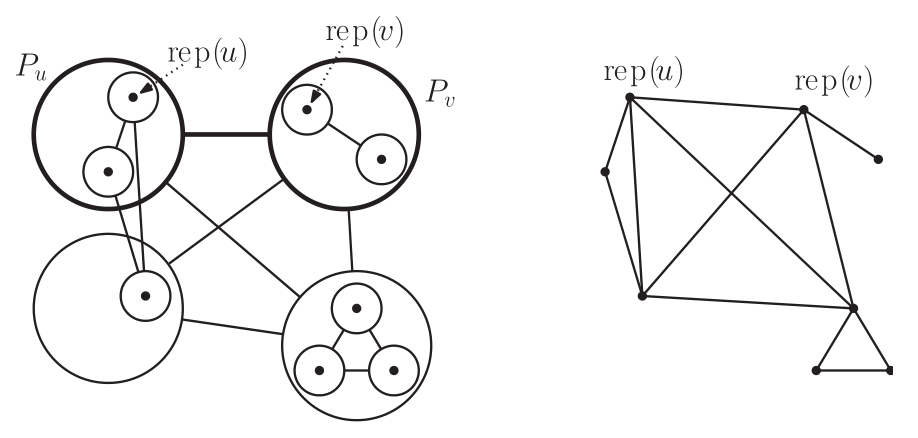
\includegraphics[width=0.8\textwidth]{figures/wspd.png}
    \caption{The well-separated pair decomposition of a set of vertices and its corresponding spanner. (Source: lecture `Geometric Spanners and Well Separated Pair Decompositions' from the course Geometric Algorithms at University of Technology Eindhoven)}
    \label{fig:wspdExample}
\end{figure}

\subsection{Yao graph and \texorpdfstring{$\Theta$}{Theta}-graph}

The Yao graph \cite{yao1982constructing} and $\Theta$-graph \cite{clarkson1987approximation} algorithms are \emph{cone-based} spanner algorithms; for each vertex $v$, they subdivide the space into $k$ non-overlapping cones (each of angle $2 \pi / k$) and connect to a certain vertex in each cone.

In the Yao graph algorithm, the nearest neighbors in each cone are connected to $v$. The $\Theta$-graph is slightly more sophisticated; it connects the vertex whose projection on the cone bisector is closest to $v$. This approach, though seemingly more unnatural, lends itself to an efficient scanning algorithm that runs in $O(n \log n)$ time. 

The Yao graph and $\Theta$-graph have similar properties. The dilation ratio of the Yao graph is bounded by $1 / (\cos \theta - \sin \theta)$ (where $\theta = 2 \pi / k$). The same bound applies to the $\Theta$-graph when $k \ge 9$.

\subsection{Greedy spanner on pruned edge set}

After performing some of the experiments we noticed that the $\Theta$-graph and Yao graph produce many unnecessary edges (refer to Section \ref{sec:results:dilation}). The greedy spanner is better at only using the edges it really needs, but is slow because it has to perform fairly expensive computations on each of the $O(n^2)$ node pairs. This leads to the idea of first executing a fast spanner, such as the $\Theta$-graph, which outputs a number of edges much smaller than $\frac{1}{2}n(n-1)$ and then running the greedy spanner on only this set of edges. This should result in the combination of the advantages of the two algorithms: a much faster algorithm but without the expense of having many redundant edges. The drawback is that the bound on the dilation ratio is no longer guaranteed by the greedy algorithm because it does not consider some (hopefully many) edge pairs. We did not perform an analysis to prove a new bound, although we did experimentally analyze it and have shown that the bound is indeed violated in some cases.

\section{Measures}
\label{sec:measures}

In the experimentation we test the following measures of the resulting spanners:

\begin{enumerate}
	\item Size (number of edges) and total weight. These are the most straightforward measures on the overall complexity of the spanner. In many applications (e.g. traffic networks) they can be used to estimate the total construction cost of the network.

	\item (Actual) stretch factor (dilation ratio). Since the parameter $t$ we are given is really only an upper bound on the stretch factor, it is possible that an algorithm will yield a spanner with a stretch factor much lower than $t$. By computing the actual value we can know how ``tight'' the algorithm is in terms of the stretch factor.

    \item Running time. We would like to analyze the running time of the algorithms and compare them to theoretical results.
\end{enumerate}

\autoref{app:metrics} describes additional metrics which we considered but that did not make it to the report.

\section{Data sets}
\label{sec:datasets}
We have run our experiments on different types of data sets to determine the performance and the quality of the spanner algorithms. For each of the data sets, we use the dilation ratios $(1.1, 1.2, 1.3, 1.5, 2, 3, 5)$.
\begin{enumerate}
	\item Uniformly distributed points. We test on data sets of 25, 50, 75, 100, 125, 150, 175, 200, 225, 250, 275, 300, 325, 350 points uniformly distributed in the area $[0,100] \times [0,100]$.
    \item Data sets from the 2013-2014 data challenge of the course Geometric
    Algorithms at University of Technology Eindhoven. The data challenge
    includes six data sets which are summarized in \autoref{tab:datasets} in
    \autoref{app:datasets}.
    As can be seen from the table, there is a great diversity in the number of vertices. Using large data sets can show the limits of the algorithms if the running time exceptionally increases. The range of the x-axis and y-axis also differ considerably. This is done to make sure that algorithms that scale the input also work for larger values.
    \item Real-world dataset. We created a mixed data set containing all train stations in The Netherlands as well as all bus stops in Eindhoven. Because we could not obtain a data set containing all bus stops, these are not the actual bus stops but rather random points in the region of Eindhoven. We scaled the 442 GPS coordinates to integers by multiplying them by $10^{4}$. The idea of the data set is to test how well the algorithm deals with points on different scales, which might break implementations that use normalizing length or that assume in some way that close pairs are distributed evenly over the map. Additionally, the map contains real and realistic data which is also interesting in its own right. We also created a similar, but smaller, map containing all train stations in Luxembourg.
\end{enumerate}

\section{Implementation}
\label{sec:implementation}
To perform experiments the algorithms were implemented in Python 2.7.3. Python is an interpreted programming language that allows for rapid development. To efficiently perform computations with large amounts of numerical data (in terms of speed and storage) NumPy 1.6.1 was used. The experiments were performed on a HP 8540w notebook with an Intel Core i5-540M 2.53GHz (dual core) processor and 4GB of RAM memory.

The algorithms were not optimized to achieve an optimal (asymptotical) running time, mainly because that is outside the scope of this study. As a consequence, the asymptotical running time of the greedy algorithm is $O(n^3 \log n)$, and that of the Yao- and $\Theta$-graph algorithms is $O(n^2 \log n)$ where $n$ is the number of vertices on which the spanner is to be computed. The implementation of the WSPD Spanner does run in $O(n \log n)$ time if the quadtree has depth $O(\log n)$ which is reasonable to assume for evenly distributed data. If the data is not evenly distributed the running time increases to $O(n^2)$ for most data but is not bounded by $n$ in the worst case.

Although the greedy spanner can handle duplicate points, these are removed from the data sets because the WSPD-spanner and the Yao and $\Theta$-graph are not able to handle duplicate points.

The algorithms were then combined in an experimentation environment which computes a spanner for each input graph using each of the algorithms with each of the chosen dilation ratios. It then computes the relevant measures and stores these for later analysis.

\subsection{Greedy Spanner}

The greedy algorithm was implemented in the most basic form: first the distances
between each node pair are computed and sorted in $O(n^2 \log n)$ time, and then
the algorithm successively checks each node pair to see if the dilation ratio between that node pair is sufficiently low. For this computation the length of the shortest path on the graph is computed using Dijkstra's algorithm, in $O(n \log n)$ time for each of the $n^2$ pairs, yielding a total running time $O(n^3 \log n )$.

\subsection{WSPD}

The implementation of the WSPD-spanner is based on a quadtree of the vertices. The quadtree is built top-down: for each level of the tree the vertices are divided into its four quadrants. This process is recursive and finishes if a quadrant has only one vertex.

An $s$-well-separated point decomposition of the vertices is computed using $s=4(t+1)/(t-1)$. The construction is done recursively by comparing different cells of the quadtree. Consider two cells $u$ and $v$ which are at an equal height or the depth of $v$ is greater than the depth of $u$. If they are well-separated, which is checked by considering their axis aligned bounding boxes, the pair is outputted. If they are not well-separated, we consider the children of cell $u$ and apply the procedure to $\{u_i,v\}$ for each of the four children $u_i$ of $u$. If $u$ has only one point while $v$ has multiple points we instead recurse on the children of $v$.

Caution must be taken to prevent duplicate WSPD-pairs. When the two cells $u$ and $v$ that are considered are the same, only eight recursive calls should be made instead of the 16 recursive calls in other cases.


\subsection{Yao graph and \texorpdfstring{$\Theta$}{Theta}-graph}

We implement a na{\"i}ve algorithm for finding the Yao graph. For each vertex $v$, we iterate each vertex $u$ other than $v$ and find the cone $u$ is in and the distance between $u$. An edge is created between $v$ and the nearest vertex in each cone along the way. The total running time is $O(n^2)$.

The $\Theta$-graph algorithm is implemented in a similar way, but instead of finding the distances from $u$ to $v$, we find the distance from $u$ to the projection of $v$ on the cone bisector. See \autoref{fig:thetaYao} for a graphical illustration. The running time is also $O(n^{2})$.

\begin{figure}[h]
    \centering
    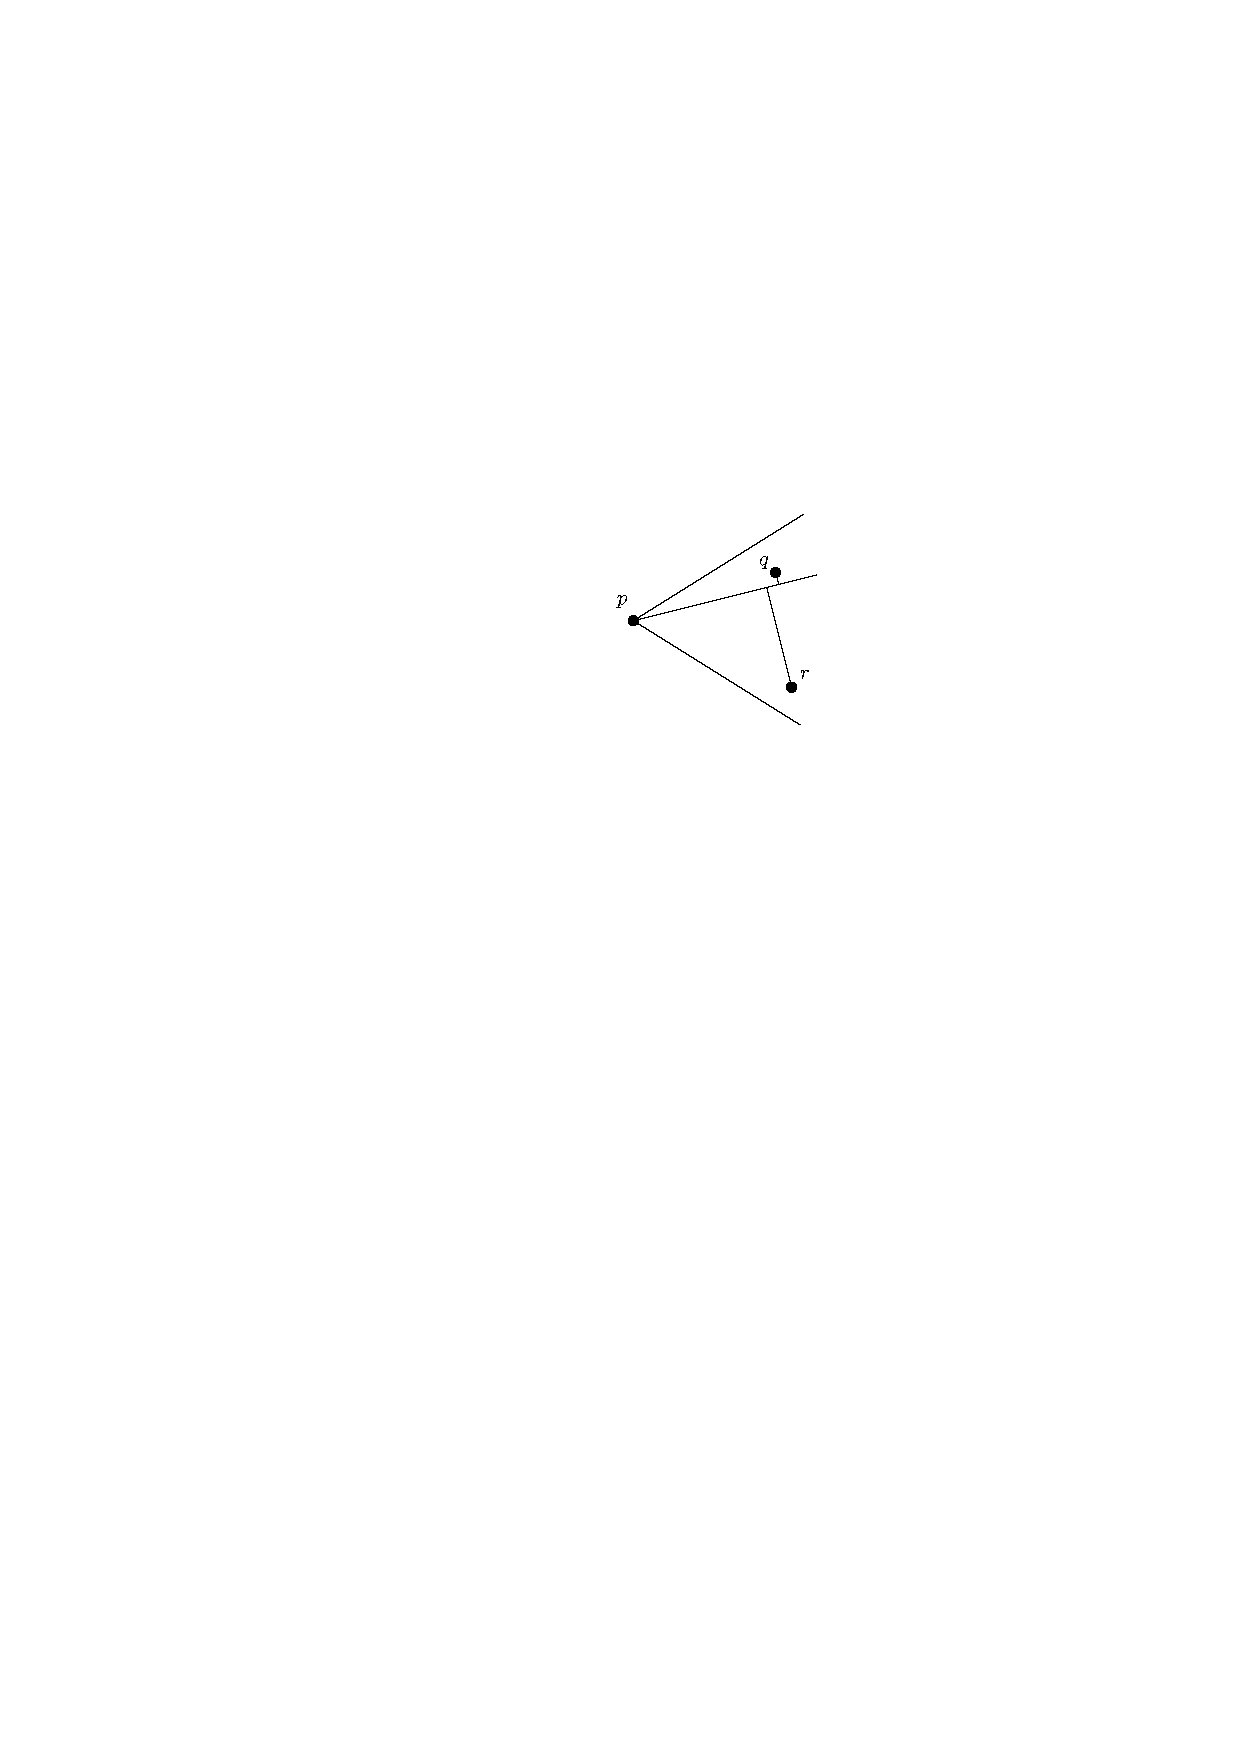
\includegraphics[width=0.4\textwidth]{figures/Theta.pdf}
    \caption{Vertex $p$ in the cone is connected to $q$ in the Yao graph while it is connected to $r$ in the Theta graph.}
    \label{fig:thetaYao}
\end{figure}

\subsection{Greedy spanner on pruned edge set}

The implementation of this algorithm simply consists of first computing the $\Theta$-graph and then computing the greedy spanner, with the exception that it operates only on node pairs that were output by the $\Theta$-graph instead of on all node pairs.

\section{Experiment Results}
\label{sec:results}
The experiments have been performed as described in the previous sections. This
section describes and discusses the results that were obtained.

Because of the rapid increase of the running time with the number of vertices in
the input set, a number of experiments were computationally unfeasible. The
greedy algorithm was not executed for input graphs of more than 450 vertices and
the Yao- and $\Theta$-graph algorithms were not executed for input graphs of
more than 3000 vertices with the exception of the data challenges. See
\autoref{tab:dataChallengeResults} in \autoref{app:dataChallengeResults} for the
results of the data challenge using the $\Theta$-graph.

\subsection{Running time}
\label{sec:results:runningtime}

\subsubsection{Running time vs.\ size of input graph}

As expected from the asymptotic running times, the greedy algorithm is much slower than the Yao and $\Theta$-graph algorithms, which perform nearly identically. This is depicted in \autoref{fig:runningtime}. \autoref{fig:runningtime_wo_greedy} shows the same data, but with the greedy algorithm left out and scaled vertically. Surprisingly, the WSPD algorithm is the slowest of those four algorithms. The Greedy Theta algorithm is approximately a factor 100\% (for small datasets) to 30\% (for large datasets) slower than the $\Theta$-graph. It can  be seen that the $\Theta$-graph algorithm is slightly faster than the Yao algorithm, which is probably due to the fact that computing the distance along the bisector is computationally cheaper than computing the Euclidean distance.

For datasets of 10,000 points the $\Theta$-graph was computed in 468 seconds for dilation ratio 1.5.

\begin{figure}[h]
    \begin{minipage}[t]{0.42\textwidth}
        \centering
        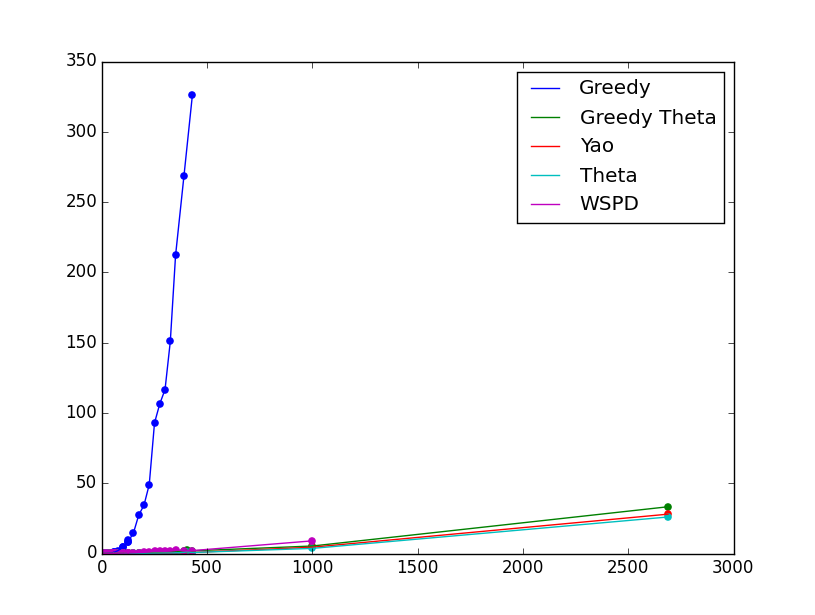
\includegraphics[width=\textwidth]{figures/Running_time_vs_number_of_vertices}
        \caption{Running time of the five algorithms on input graphs with various amount of edges, for dilation ratio 1.5.}
        \label{fig:runningtime}
    \end{minipage}
    \hfill
    \begin{minipage}[t]{0.54\textwidth}
        \centering
        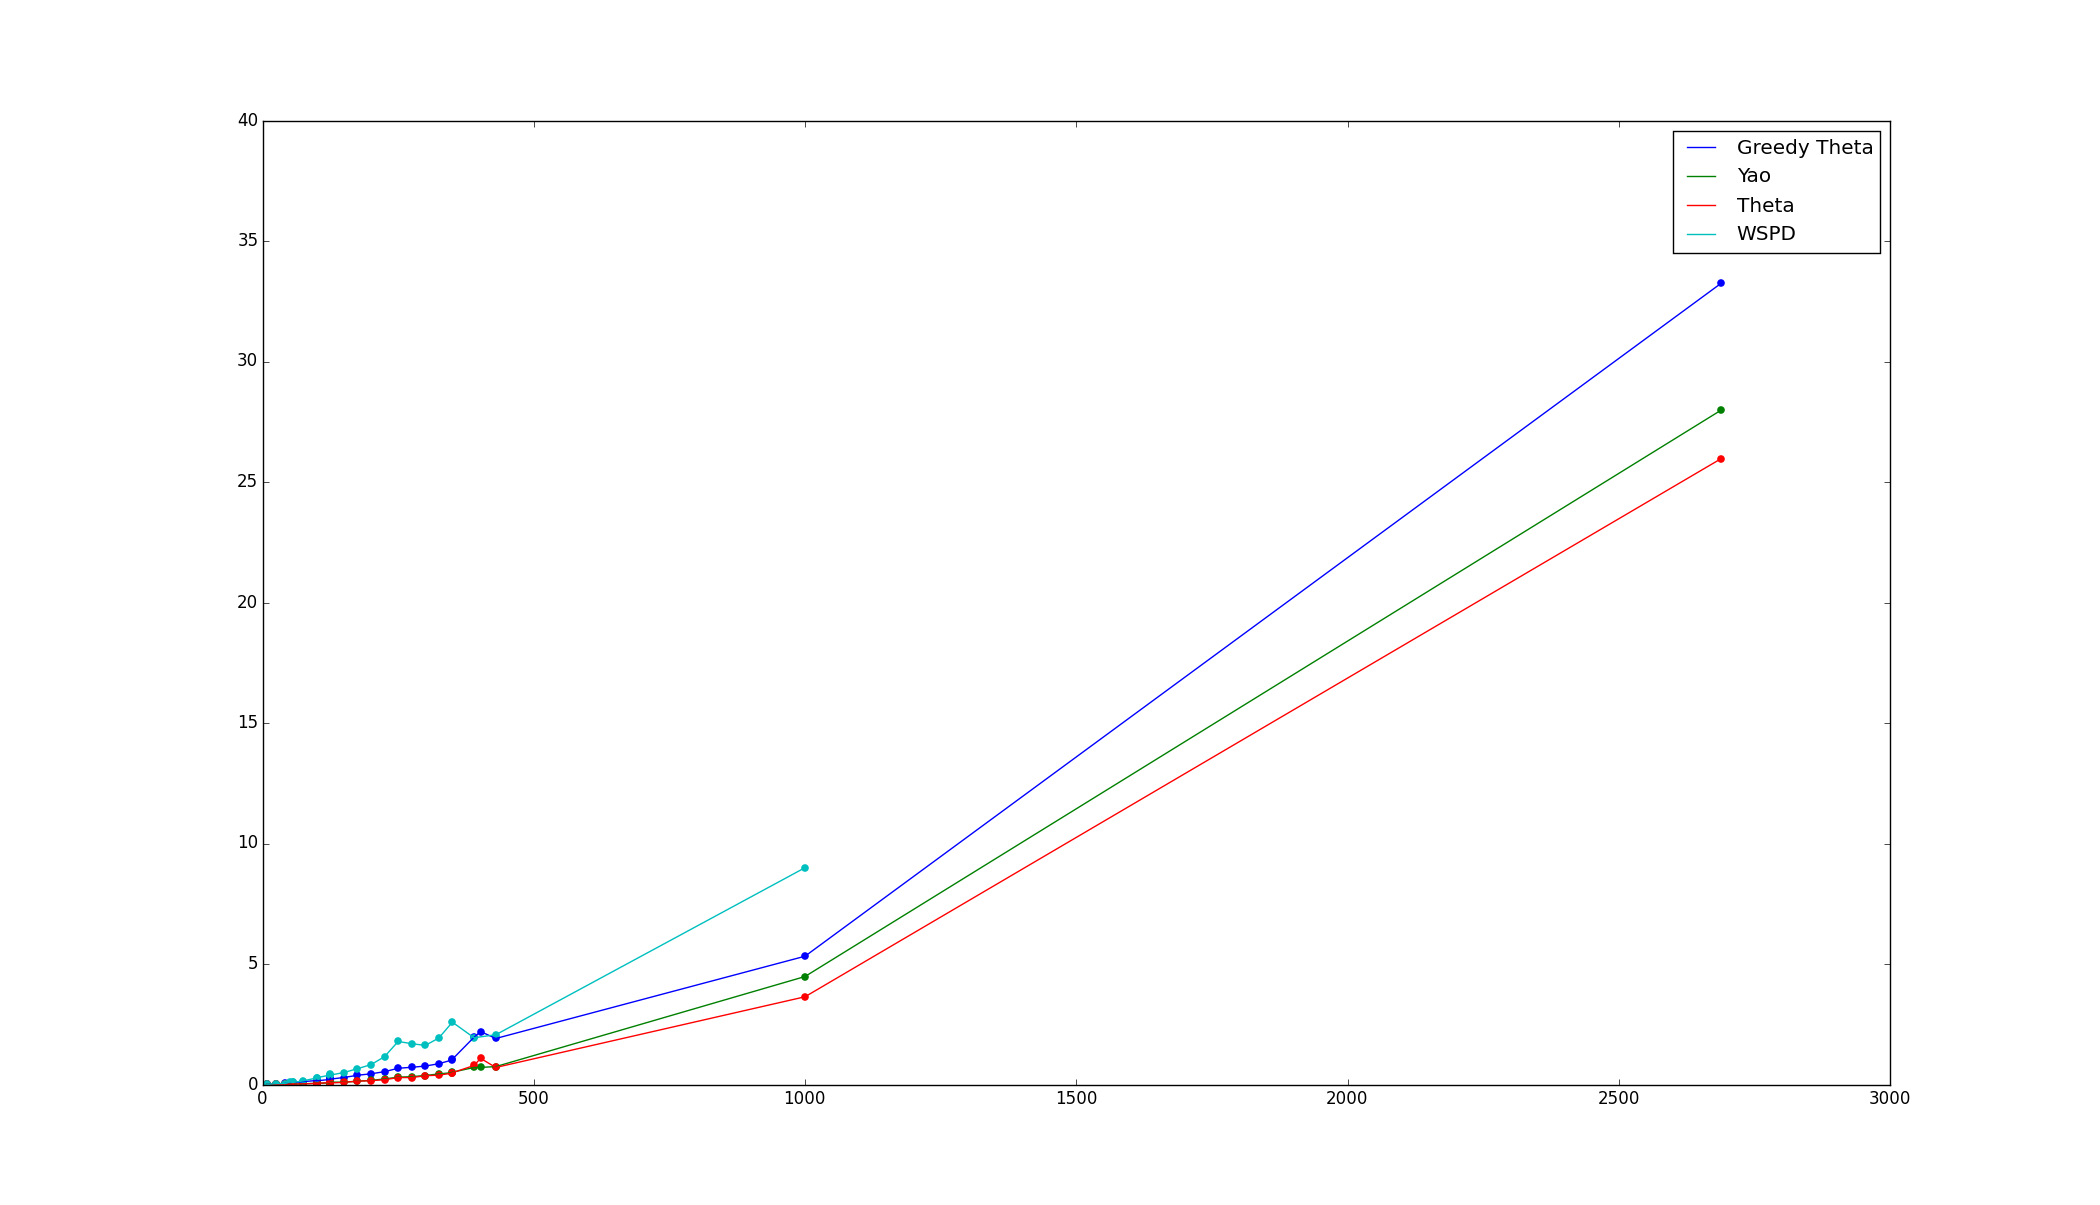
\includegraphics[width=\textwidth]{figures/Running_time_vs_number_of_vertices_wo_greedy}
        \caption{The same graph, with the greedy spanner excluded.}
        \label{fig:runningtime_wo_greedy}
    \end{minipage}
\end{figure}

\subsubsection{Running time vs.\ required dilation ratio}

The running time depends not only on the size of the input graph, but also on the dilation ratio. This relation is depicted in \autoref{fig:speed_vs_dilation}. The running time for the greedy algorithm is not shown to allow for a more detailed view on the others. It has a similar shape to the curves that are depicted. It can be seen that the Greedy Theta algorithm depends the most on the dilation ratio. This is likely explainable from the fact that the running time of the Greedy Theta algorithm depends on the amount of edges of the $\Theta$-graph, which in turn depends on the dilation ratio (see section \ref{sec:edges_vs_dilation}).

\begin{figure}[h]
    \centering
    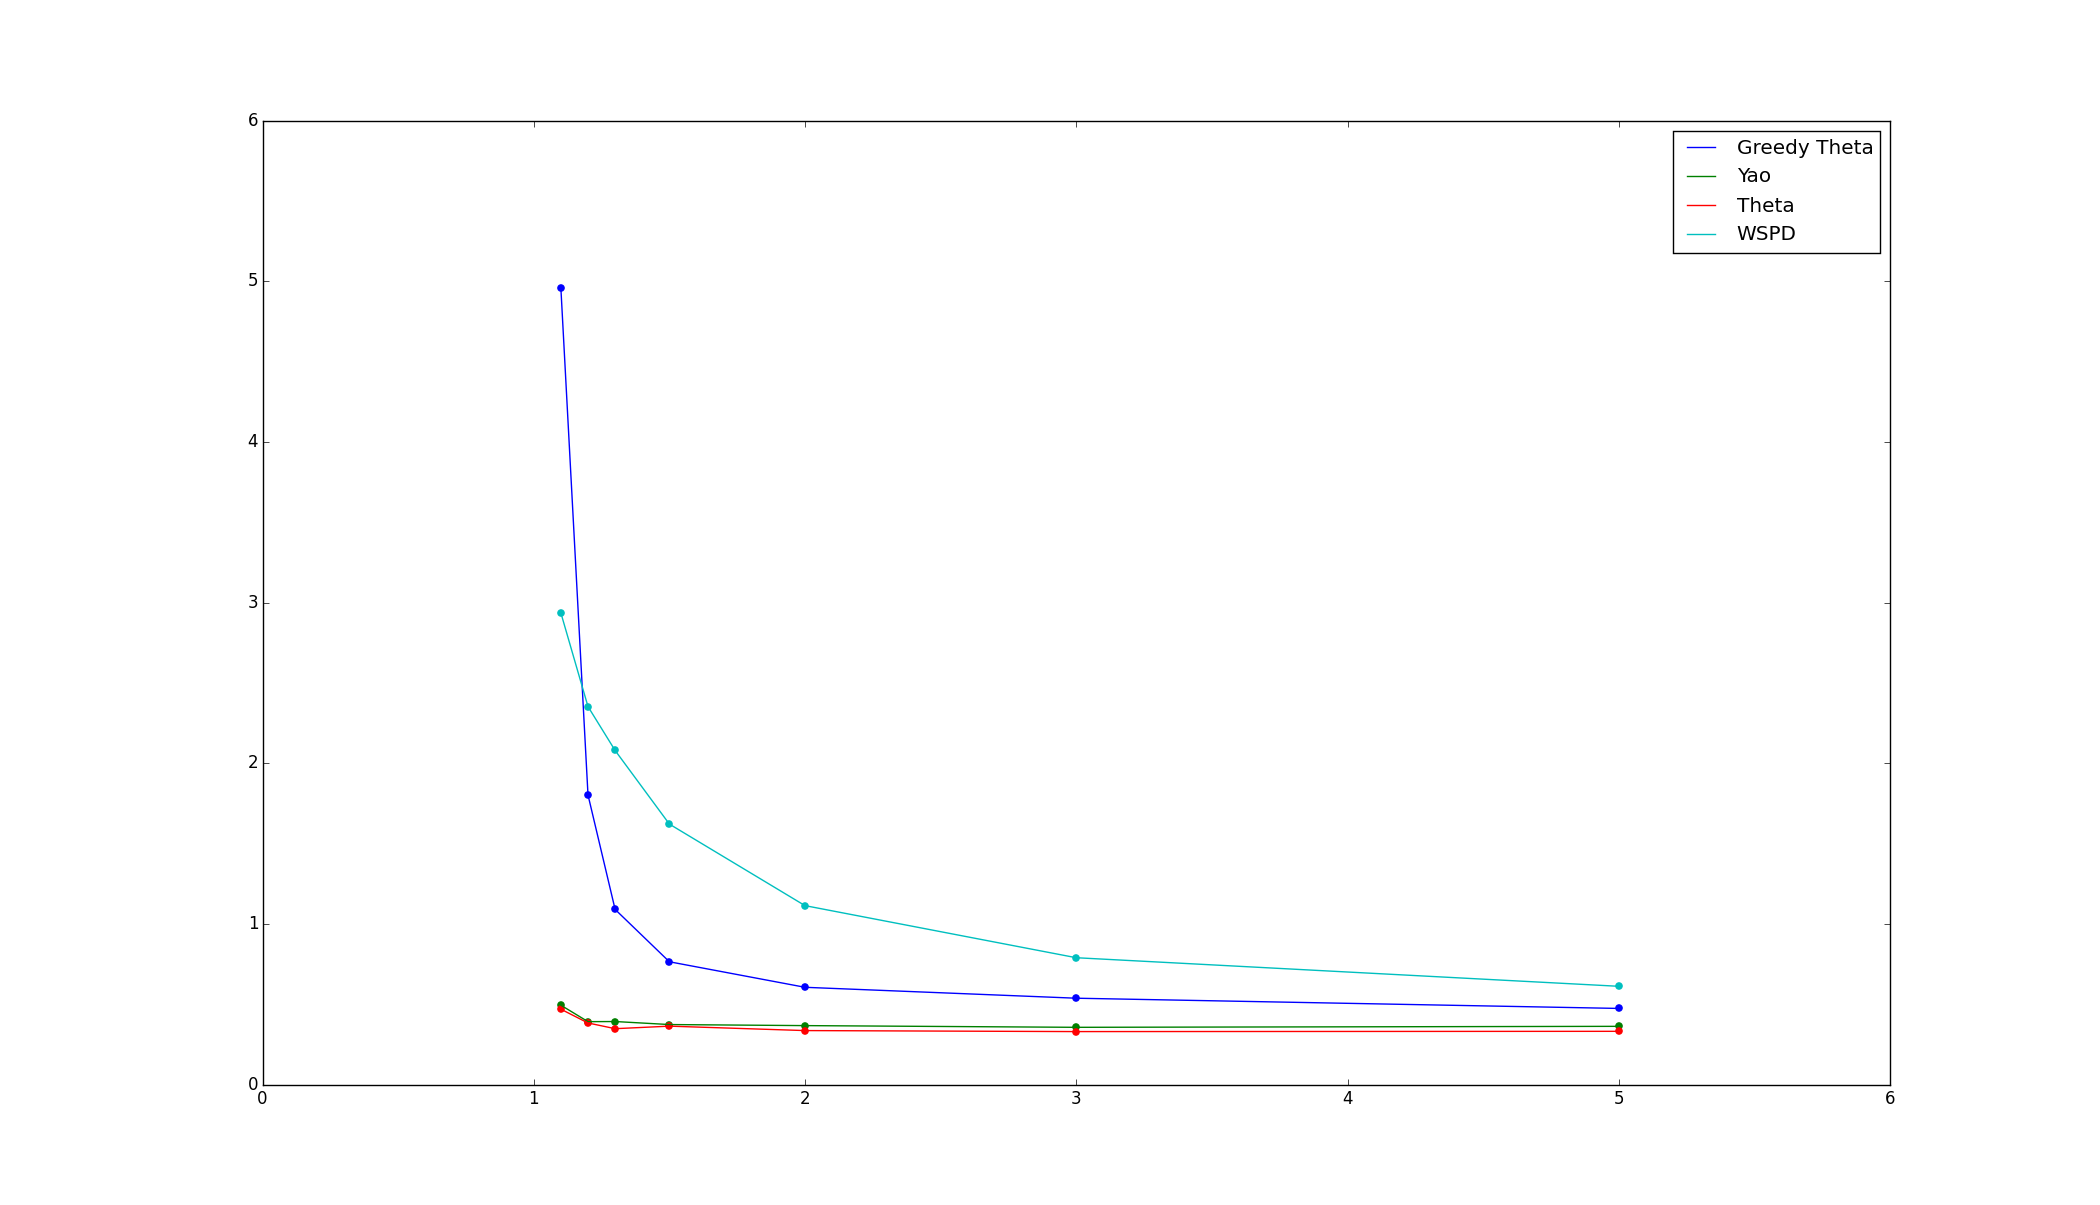
\includegraphics[width=\textwidth]{figures/Running_time_vs_dilation_wo_greedy}
    \caption{Running time of the Greedy Theta, Yao, $\Theta$ and WSPD algorithms on input graphs with 300 vertices, for various dilation ratios.}
    \label{fig:speed_vs_dilation}
\end{figure}

\subsection{Number of edges}
\label{sec:results:nredges}

\subsubsection{Number of edges vs.\ number of vertices}
\label{sec:edges_vs_vertices}

Except for the WSPD spanner algorithm, the number of edges forms roughly a linear relation with the number of vertices in the input set, as is depicted in \autoref{fig:nredges}. The graphs for the Yao and $\Theta$-graphs almost coincide as can be seen in \autoref{fig:nredges-no-wspd}, because of how they introduce new edges (refer to \autoref{sec:algorithms}). Those for the greedy and greedy-$\Theta$ also almost coincide.

In this example, which shows all spanners with required dilation ratio 5, the greedy spanner uses about as many edges as there are vertices in the input graph and the Yao and $\Theta$-graph spanners use about 3 times as many edges as there are vertices in the input graph. This is inherent to the way the Yao and $\Theta$-graph spanners are constructed, as is discussed in  \autoref{sec:results:dilation}.

\begin{figure}[h]
	\begin{minipage}[t]{0.48\textwidth}
      \centering
      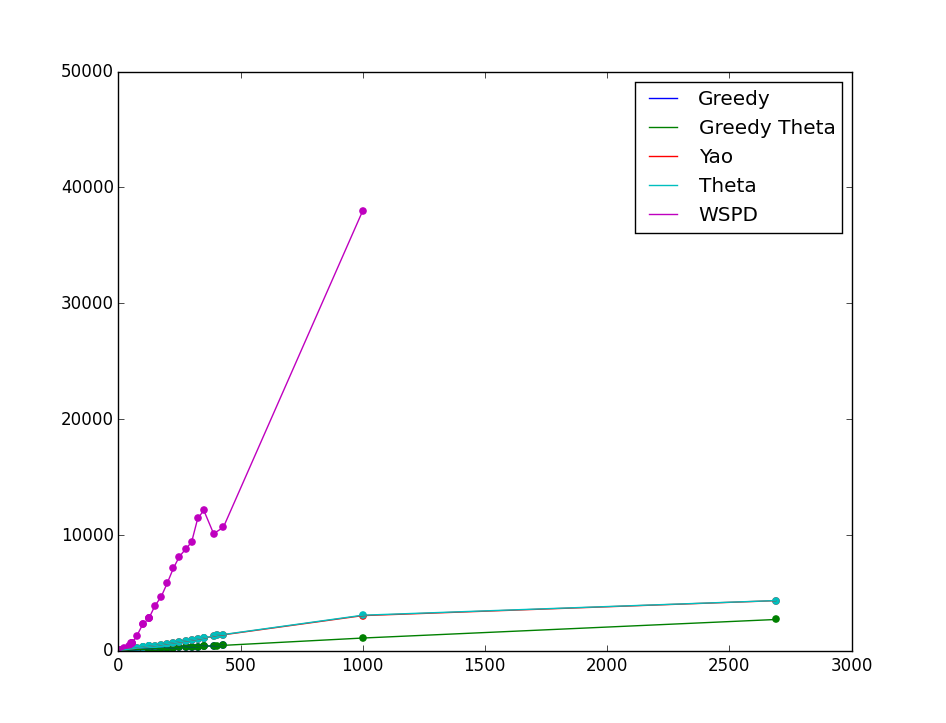
\includegraphics[width=\textwidth]{figures/Number_of_vertices_vs_number_of_edges.png}
      \caption{Number of edges of spanners generated by the different algorithms on input graphs of various sizes, all with required dilation ratio 5.}
      \label{fig:nredges}
    \end{minipage}
    \hfill
    \begin{minipage}[t]{0.48\textwidth}
      \centering
      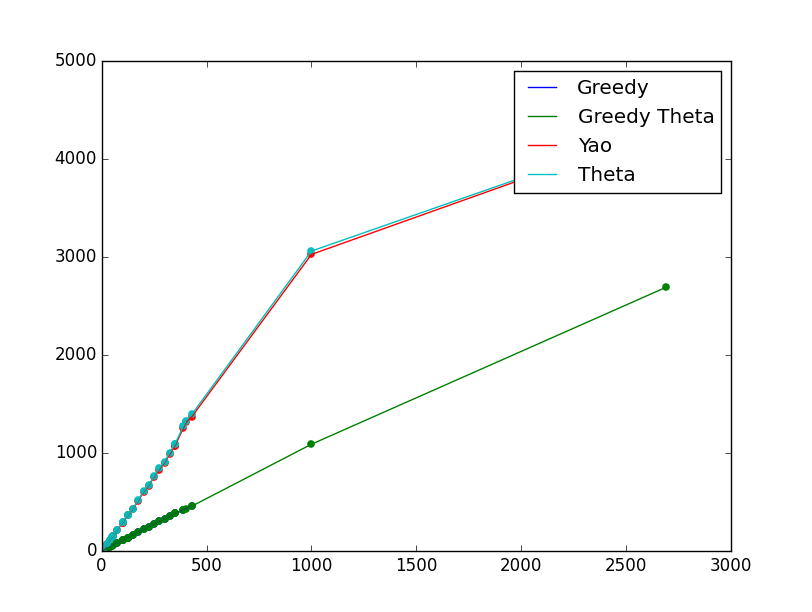
\includegraphics[width=\textwidth]{figures/Number_of_vertices_vs_number_of_edges_no_WSPD.png}
      \caption{The same graph, with WSPD excluded.}
      \label{fig:nredges-no-wspd}
    \end{minipage}
\end{figure}

\subsubsection{Number of edges vs.\ required dilation ratio}
\label{sec:edges_vs_dilation}

Figures \ref{fig:nedges_vs_t_random_300} and \ref{fig:nedges_vs_t_dc2} show the relationship between the number edges vs.\ the required dilation ratio. As the required dilation ratio increases the number of edges tends to decrease.

\begin{figure}[h]
    \begin{minipage}[t]{0.48\textwidth}
      \centering
      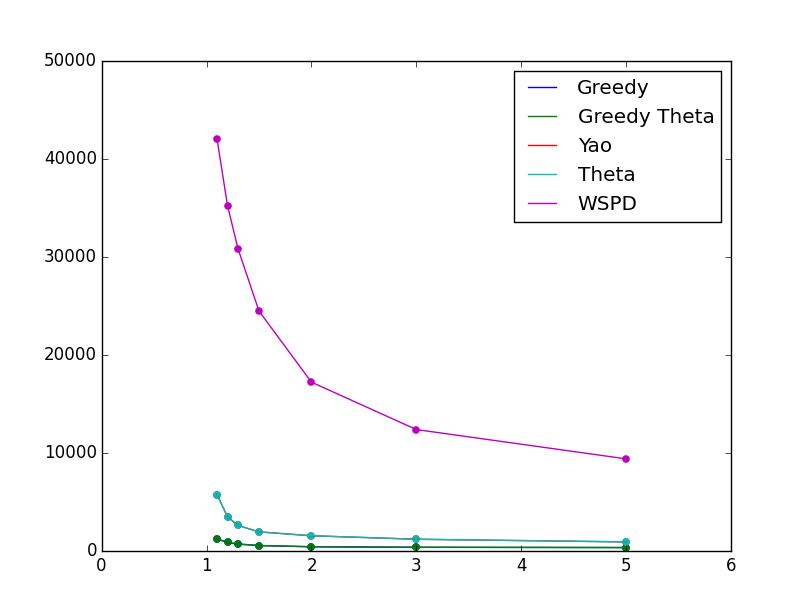
\includegraphics[width=\textwidth]{figures/nedges_vs_t_random_300}
      \caption{Number of edges vs.\ dilation ratio on the ``random 300'' data set.}
      \label{fig:nedges_vs_t_random_300}
    \end{minipage}
    \hfill
	\begin{minipage}[t]{0.48\textwidth}
      \centering
      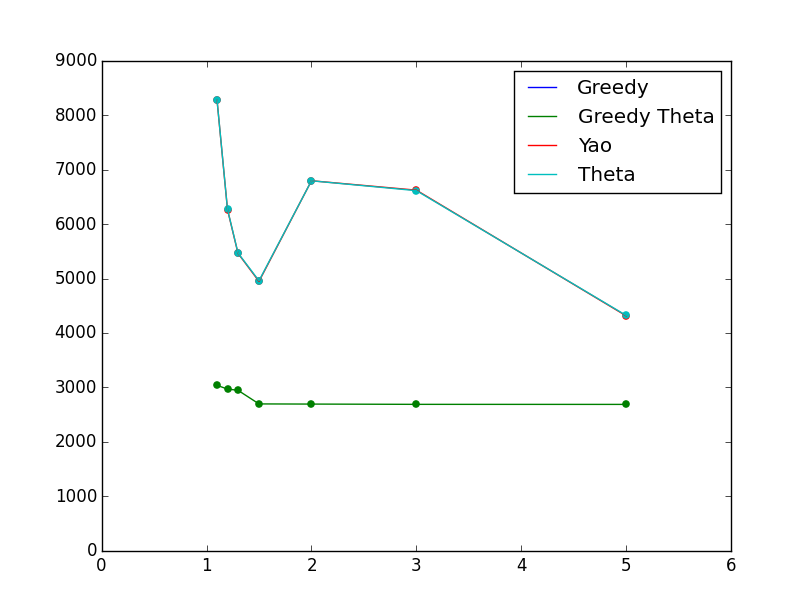
\includegraphics[width=\textwidth]{figures/nedges_vs_t_dc2}
      \caption{Number of edges vs.\ dilation ratio on the ``data challenge 2'' data set.}
      \label{fig:nedges_vs_t_dc2}
    \end{minipage}
\end{figure}

However, there is a curiosity with the Yao and $\Theta$-graph, namely when the required dilation ratio increases the number of edges sometimes \emph{increases}. This can be explained as follows: although the number of edges is always bounded by $nk$, the upper bound is hardly tight due to the phenomena of ``mutual connections'' - namely pairs of vertices $(u, v)$ such that $u$ is connected to $v$ in one of $v$'s cones and vice versa - whose frequency depends very much on the shape of the data set and the choice of $k$. This is especially evident with data sets that have a regular shape, e.g. with the ``data challenge 2'' data set. See \autoref{fig:yao-dc-1.5} and \autoref{fig:yao-dc-2}. With $t = 1.5$ ($k = 11$) a lot of horizontal mutual connections are possible, but with $t = 2$ ($k = 8$) they no longer are, resulting in an increase of the number of edges.

\begin{figure}[h]
    \begin{minipage}[t]{0.48\textwidth}
        \centering
        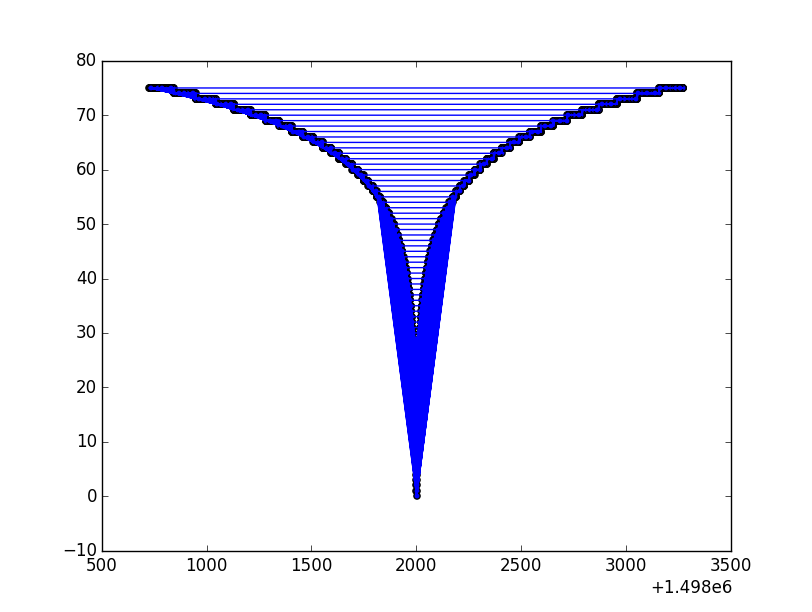
\includegraphics[width=\textwidth]{figures/theta-dc-1_5}
        \caption{$\Theta$-graph on the ``data challenge~2'' data set with $t = 1.5$ ($k = 11$). $|E| = 4950$.}
        \label{fig:yao-dc-1.5}
    \end{minipage}
    \hfill
    \begin{minipage}[t]{0.48\textwidth}
        \centering
        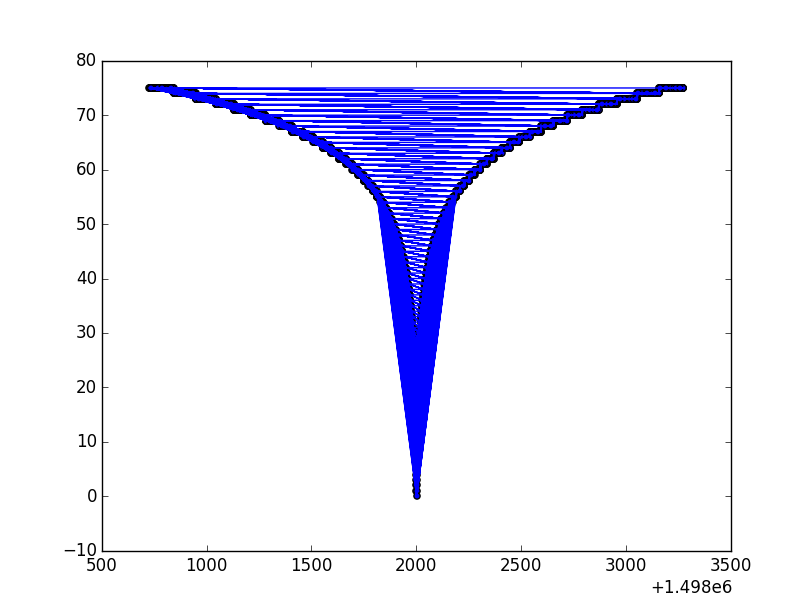
\includegraphics[width=\textwidth]{figures/theta-dc-2}
        \caption{$\Theta$-graph on the ``data challenge~2'' data set with $t = 2$ ($k = 8$). $|E| = 7342$.}
        \label{fig:yao-dc-2}
    \end{minipage}
\end{figure}

\subsection{Actual dilation ratio}
\label{sec:results:dilation}

The required dilation ratio is a parameter to the algorithms. However that does not mean the algorithms produce a spanner with exactly that dilation ratio. Usually the dilation ratio will be slightly smaller, sometimes even much smaller. This is in itself not a problem, a smaller dilation ratio can in fact be considered better than a larger one, but it is also unnecessary so it should not come at the expense of other measures, such as the amount of edges and the running time.

Figure \ref{fig:actual_vs_required_dilation} shows the actual dilation ratio of all constructed spanners vs.\ the required dilation ratio that was provided to the algorithm as a parameter. The reference line $y = x$ is also drawn. The greedy algorithm produces spanners that have a dilation ratio close to the required dilation ratio in all cases. The Yao and $\Theta$-graph and WSPD algorithm, on the other hand, produce only spanners with a dilation ratio smaller than 2. Notice how the greedy-$\Theta$ algorithm \emph{violates} the required dilation ratio.

\begin{figure}[h]
    \centering
    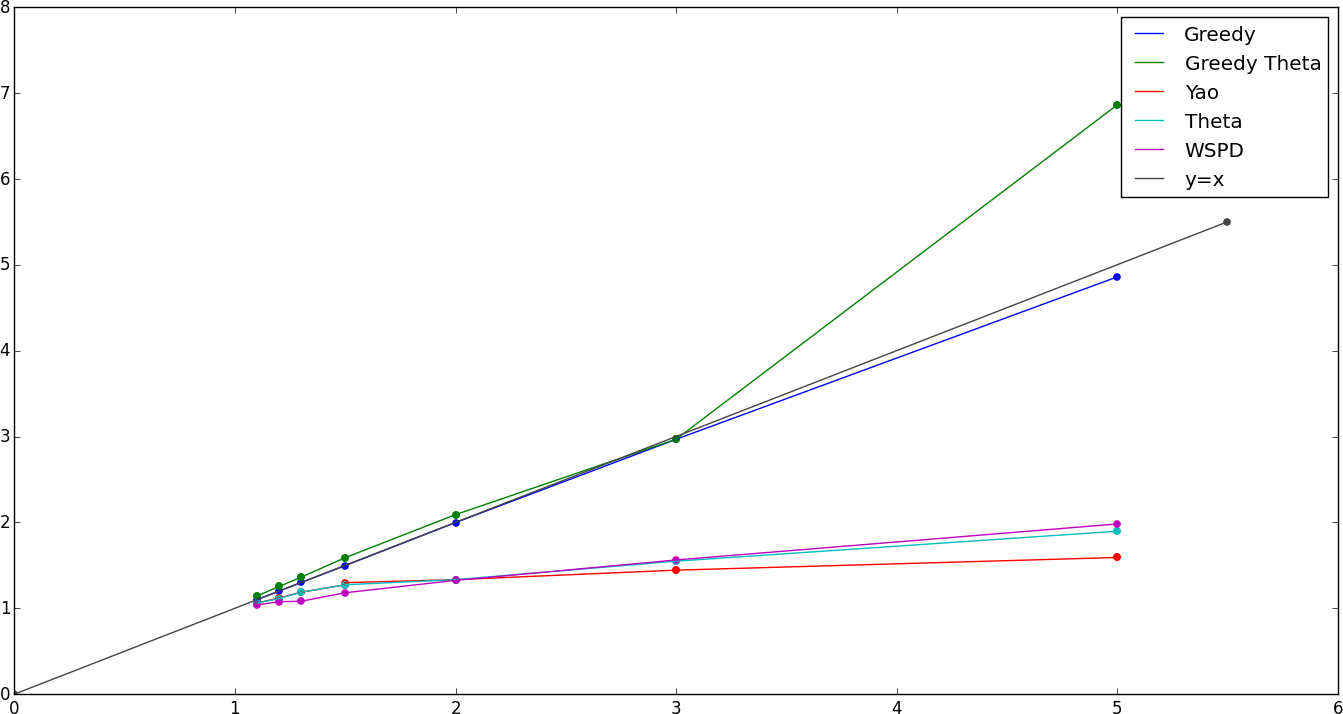
\includegraphics[width=\textwidth]{figures/actual_dilation_vs_required}
    \caption{Actual dilation ratios of generated spanners on the ``Dutch train station'' data set for each required dilation ratio.}
    \label{fig:actual_vs_required_dilation}
\end{figure}

Figures \ref{fig:greedy_100_dilation} and \ref{fig:yao_100_dilation} show spanners constructed by the greedy algorithm and by the Yao algorithm for the ``random 100'' data set. The Yao spanner has many more edges than the greedy spanner (as is discussed in Section \ref{sec:results:nredges}). But what is also very well visible here is that each vertex in the Yao spanner must have a neighbor 'in each direction', so to speak. This means that every vertex in the Yao spanner will have a relatively high degree: the maximum degree for this example is 12. This is opposed to the greedy spanner, which has a maximum degree of 4 and where many vertices are on paths connecting vertices that are close to each other. These vertices have a degree of only two or even one for the endpoints of these paths. This observation explains why Yao spanners have a relatively high amount of edges and also a low dilation ratio, even when a low dilation ratio is not required.

\begin{figure}[h]
    \begin{minipage}[t]{0.48\textwidth}
        \centering
        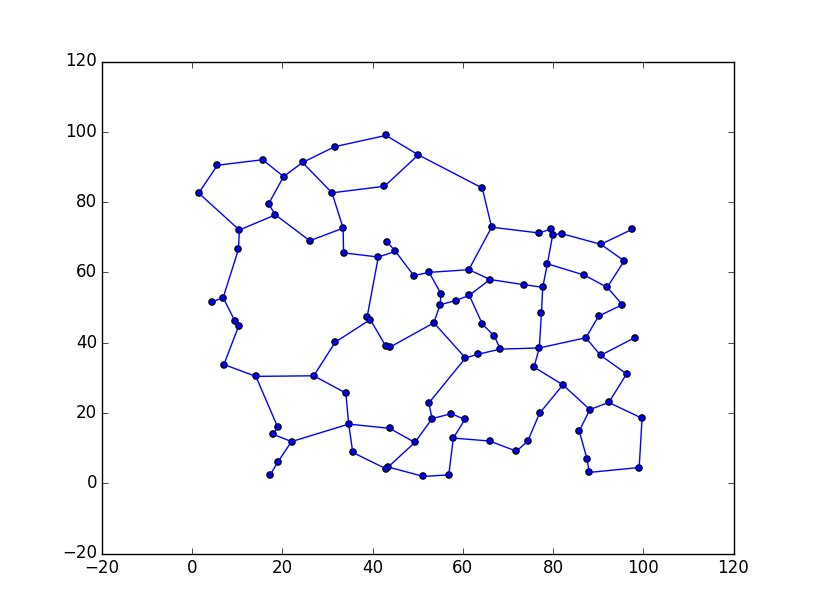
\includegraphics[width=\textwidth]{figures/greedy_100_points_dilation_3}
        \caption{Greedy spanner with $t$ = 3.}
        \label{fig:greedy_100_dilation}
    \end{minipage}
    \hfill
    \begin{minipage}[t]{0.48\textwidth}
        \centering
        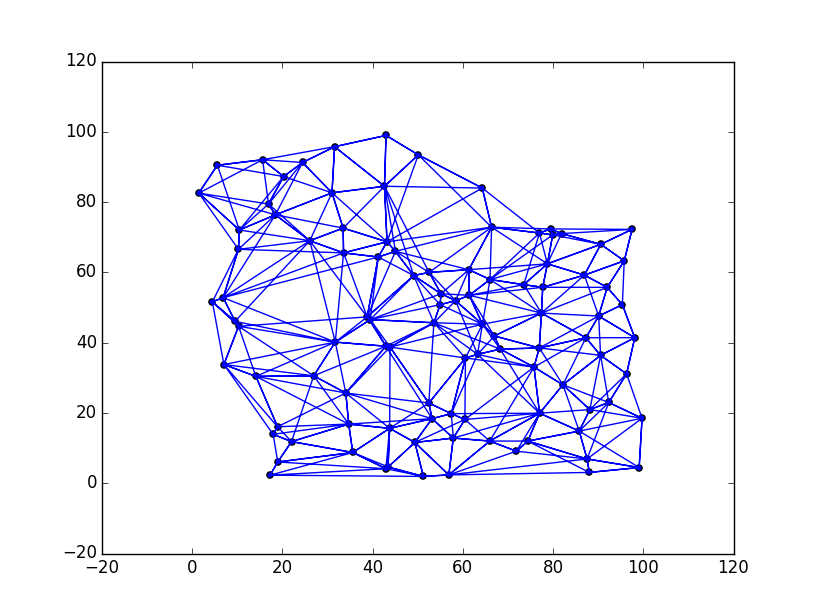
\includegraphics[width=\textwidth]{figures/yao_100_points_dilation_3}
        \caption{Yao graph with $t$ = 3.}
        \label{fig:yao_100_dilation}
    \end{minipage}
\end{figure}


\section{Conclusion}
\label{sec:conclusion}
In this paper we have compared experimental results of five geometric spanner algorithms. The algorithms that were implemented are the greedy spanner, the Yao graph, the $\Theta$-graph, a spanner based on well-separated point decompositions and a heuristic that combines the $\Theta$-graph and the greedy spanner. We have considered the size, actual stretch factor and running time. We tested on randomly distributed data sets, two real-world data sets with train stations in the Netherlands and Luxembourg and six data sets from a data challenge for geometric spanners. 

The experiments show that the greedy spanner has considerably less edges than both the Yao and $\Theta$-graph. A result of the high number of edges is that the vertices in the Yao and $\Theta$-spanners have a relatively high degree compared to the greedy spanner where many edges are on a path.  The disadvantage of the good quality of the greedy spanner is the high running time. While the Yao and $\Theta$-graph have a running time of $O(n^2)$, the greedy spanner needs $O(n^3 \log n)$. We furthermore found that the greedy spanner has a dilation ratio close to the required dilation ratio while the Yao and $\Theta$-algorithms only produce spanners with dilation ratio smaller than 2, a consequence of the Yao and $\Theta$-algorithms adding more edges than necessary. The metrics of the heuristic algorithm are a mixture of its two godfathers; it has slightly more edges than the greedy algorithm but runs only slightly slower than the $\Theta$-graph. It does not guarantee a certain dilation ratio, however. The WSPD algorithm is completely eclipsed by the $\Theta$-graph in this study, it is slower and performs worse on the evaluated metrics.


%\bibliographystyle{alpha}
\bibliographystyle{plain}
\bibliography{literature}
\newpage
\appendix
\section{Appendix - Additional metrics}
\label{app:metrics}

In addition to the metrics described in \autoref{sec:measures}, a number of other metrics were proposed in the research proposal, implemented and (partially) evaluated but did not make it to the report. These are:

\begin{enumerate}
	\item Maximum degree of vertices. This measure reflects the local complexity of the spanner; a low maximum degree often reflects high resilience of the network. For instance, in communication networks, the total throughput and bandwidth at a given vertex is often bounded, and it is often desirable to have spanners where the edges are more spread apart instead of concentrating on a few vertices.

    \item Number of intersections. This measure is an aspect of the overall complexity of the spanner. For instance, if the spanner is to be visualized, a smaller number of intersections leads to better readability. In wireless communication networks, a smaller number of intersections means less signal interference.

	\item Maximum eccentricity (diameter) and average eccentricity of resulting spanner. For some applications, fewer hops in the network are desirable. Such applications include wired or wireless communication networks and transportation networks.
\end{enumerate}

These measures were removed from our study for three reasons: firstly, much of the variance in the measured values on these metrices is explained by the number of edges in the spanner and we did not study the reasons that explain the remainder of the variance; secondly, we did not find any specialist algorithms that explicitly focus to score well on one of these metrics and thirdly, this report is subject to a page limit and including these metrics would mean that we could write less thoroughly on the other metrics.

\section{Appendix - Data sets from the data challenge}
\label{app:datasets}

\autoref{tab:datasets} shows the properties of the different data challenges.

\begin{table}[h!]
\centering
\begin{tabular}{c |c| c | c | c | c | c}
	Data set & Number of vertices & Dilation ratio & $X_{Min}$ & $X_{Max}$ & $Y_{Min}$ & $Y_{Max}$ \\ \hline
	B1 & 8 & 2.00 & 0 & 14 & 0 & 3\\
    B2 & 2,689 & 2.00 & 1,498.728 & 1,501,272 & 0 & 75\\
    B3 & 10,001 & 1.42 & 1 & 5,001 & 1 & 5,001\\
    B4 & 1,000 & 1.10 & 0 & 1,330 & 0 & 1,333\\
    B5 & 42 & 1.25 & 54 & 520 & 37 & 911\\
    B6 & 10,000 & 1.10 & 85,000 & 214,999 & 100,000 & 199,999\\
\end{tabular}
\caption{Data sets from the data challenge}
\label{tab:datasets}
\end{table}
\newpage
\section{Appendix - Results of the data challenge}
\label{app:dataChallengeResults}
\autoref{tab:dataChallengeResults} shows the number of edges and the actual
dilation ratios of the spanners generated by the $\Theta$-graph for the
different data challenges.
\begin{table}[h!]
\centering
\begin{tabular}{c |c| c | c | c }
	Data set & \#vertices & Required dilation ratio & Actual dilation ratio
	& \#edges  \\ \hline 
	B1 & 8 & 2.00 & 1.4 & 15 \\
    B2 & 2,689 & 2.00 & 1.34 & 6,795 \\
    B3 & 10,001 & 1.42 & 1.12 & 51,528 \\
    B4 & 1,000 & 1.10 & 1.05 & 20,772 \\
    B5 & 42 & 1.25 & 1.08 & 318  \\
    B6 & 10,000 & 1.10 & 1.08 & 335,985 \\
    Train stations NL & 442 & 1.30 & 1.14 & 3.972 \\
\end{tabular}
\caption{Results of the data challenge using the $\Theta$-graph.}
\label{tab:dataChallengeResults}
\end{table}

\end{document}
